Note on universal properties: When dealing with categories, we are fundamentally dealing with abstractions that behave alike to a known construction. These behaviours are made precise by the use of a \emph{universal property}. We illustrate this with the definition of a (co)product: 

\begin{definition}\label{app:def:product_coproduct}
  Let $\CC$ be a category and $x,y \in ob(\CC)$. Their \emph{\green{product}} is an object $x \prod y$ in $\CC$ with morphisms $\pi_x : x \prod y \to x$ and $\pi_y : x \prod y \to y$. Their \emph{\green{coproduct}} is defined as the object $x \coprod y$ together with the maps $\iota_x : x \to x \coprod y$ and $\iota_y : y \to x \coprod y$. Both of these definitions are universal with their properties. 
  % https://q.uiver.app/#q=WzAsOCxbMSwxLCJ4IFxccHJvZCB5Il0sWzEsMiwieCJdLFsyLDEsInkiXSxbNCwxLCJ4XFxjb3Byb2QgeSJdLFswLDAsIloiXSxbMywwLCJaXlxccHJpbWUiXSxbNCwyLCJ4Il0sWzUsMSwieSJdLFswLDEsIlxccGlfeCJdLFswLDIsIlxccGlfeSIsMl0sWzQsMiwiXFxwaV5cXHByaW1lX3kiXSxbNCwxLCJcXHBpX3heXFxwcmltZSIsMl0sWzQsMCwiXFxleGlzdHMhIiwxXSxbNyw1LCJcXGlvdGFfeSIsMl0sWzYsNSwiXFxpb3RhX3giXSxbNywzLCJcXGlvdGFfeSJdLFs2LDMsIlxcaW90YV94IiwyXSxbMyw1LCJcXGV4aXN0cyEiLDEseyJzdHlsZSI6eyJ0YWlsIjp7Im5hbWUiOiJhcnJvd2hlYWQifSwiaGVhZCI6eyJuYW1lIjoibm9uZSJ9fX1dXQ==
  \[\begin{tikzcd}
	  Z &&& {Z^\prime} && \\
	  & {x \prod y} & y && {x\coprod y} & y \\
	  & x &&& x
	  \arrow["{\exists!}"{description}, from=1-1, to=2-2]
	  \arrow["{\pi^\prime_y}", from=1-1, to=2-3]
	  \arrow["{\pi_x^\prime}"', from=1-1, to=3-2]
	  \arrow["{\pi_y}"', from=2-2, to=2-3]
	  \arrow["{\pi_x}", from=2-2, to=3-2]
	  \arrow["{\exists!}"{description}, from=1-4, to=2-5]
	  \arrow["{\iota_y}"', from=2-6, to=1-4]
	  \arrow["{\iota_y}", from=2-6, to=2-5]
	  \arrow["{\iota_x}", from=3-5, to=1-4]
	  \arrow["{\iota_x}"', from=3-5, to=2-5]
  \end{tikzcd}\]
\end{definition}

\begin{definition}[\cite{moses25}]
  A \emph{\green{fusion category}} can be restated in its vector space form as a finite set of labels (sectors?) $L$ and vector spaces $V^{ab}_c$ for all $a,b,c \in L$, as well as the isomorphisms
  \[
    F^{abc}_{d} : \bigoplus_e V^{ab}_e \otimes V^{ec}_d \to \bigoplus_e V^{ae}_d \otimes V^{bc}_e
  \]
  such that the pentagon holds:
  \begin{equation}
  \begin{gathered} % From the seminar paper, adapted after skein paper.
  \begin{tikzpicture}
    \node at (0,-0.1) {$\underset{e,f}{\bigoplus} V^{ab}_e \otimes V^{ec}_f \otimes V^{fd}_g $};
    \draw[->, black] plot coordinates{(0.4,0.5) (2.5,1.5)};
    \node at (0.9,1.3) {$id_{V_{e}^{ab}} \otimes F^{ecd}_{g}$};
    \node at (4.0,1.9)  {$\underset{e,l}{\bigoplus} V^{ab}_e \otimes V^{cd}_{f} \otimes V^{el}_g$};
    \node at (7.6, 1.1) {$F^{abl}_{g} \otimes id_{V^{cd}_{l}}$};
    \draw[->] plot coordinates{(5.5, 1.5) (7.5,0.5)};
    \node at (8.0,-0.1) {$\underset{k,l}{\bigoplus} V^{ak}_{g} \otimes V^{bl}_{k} \otimes V^{cd}_{l}$};
    \node at (-0.4, -1.2) {$F^{abc}_{f} \otimes id_{V^{fd}_{g}}$};
    \draw[->] plot coordinates{(0.4,-0.5) (1.5,-1.5)};
    \node at (1.8,-2.1) {$\underset{f,h}{\bigoplus} V^{af}_{h} \otimes V^{bc}_{f}  \otimes V^{hd}_{g}$};
    \node at (4.3, -2.5) {$F^{afd}_{g} \otimes id_{V^{bc}_{f}}$};
    \draw[->] plot coordinates {(3.5,-2.0) (4.7, -2.0)};
    \node at (6.5, -2.1) {$\underset{k,h}{\bigoplus} V^{ak}_{g} \otimes V^{bc}_{h} \otimes V^{hd}_{k} $};
    \node at (8.2, -1.2) {$F^{bcd}_{k} \otimes id_{V^{ak}_{g}}$};
    \draw[->] plot coordinates {(6.4, -1.5) (7.5,-0.5) };
  \end{tikzpicture}
  \label{cat:pentagon}
  \end{gathered}
  \end{equation}
\end{definition}

\subsection{TQFT}

Hmm, where does this go?

A TQFT is defined by a finite set of labels $L$, and a rule that assigns each compact cpa-space a vector space and each map between them (a cobordism) a  linea map between spaces. A TQFT is thus a functor between the category $(Bord, \sqcup, \emptyset) \to \mathrm{Vect}$.

